\chapter{DISCOVERY OF FIVE CARBON-ENHANCED METAL-POOR STARS FROM LAMOST}\label{chap:introduction}




 \section{Results and discussion}\label{sec:discussions}
 
 \subsection{Chemical abundance comparison with literature data}
 
We provided stellar parameters and detailed chemical abundances 
for five metal-poor red giant stars, reported for the first time using high resolution spectroscopy. 
These stars exhibit similar chemical abundance patterns to,
reported in other, very and extremely metal-poor stars \citep[e.g.,][]{2007A&A...476..935F, 2013ApJ...762...26Y}.

\vspace{5mm}
\begin{figure}[!ht]
\centering
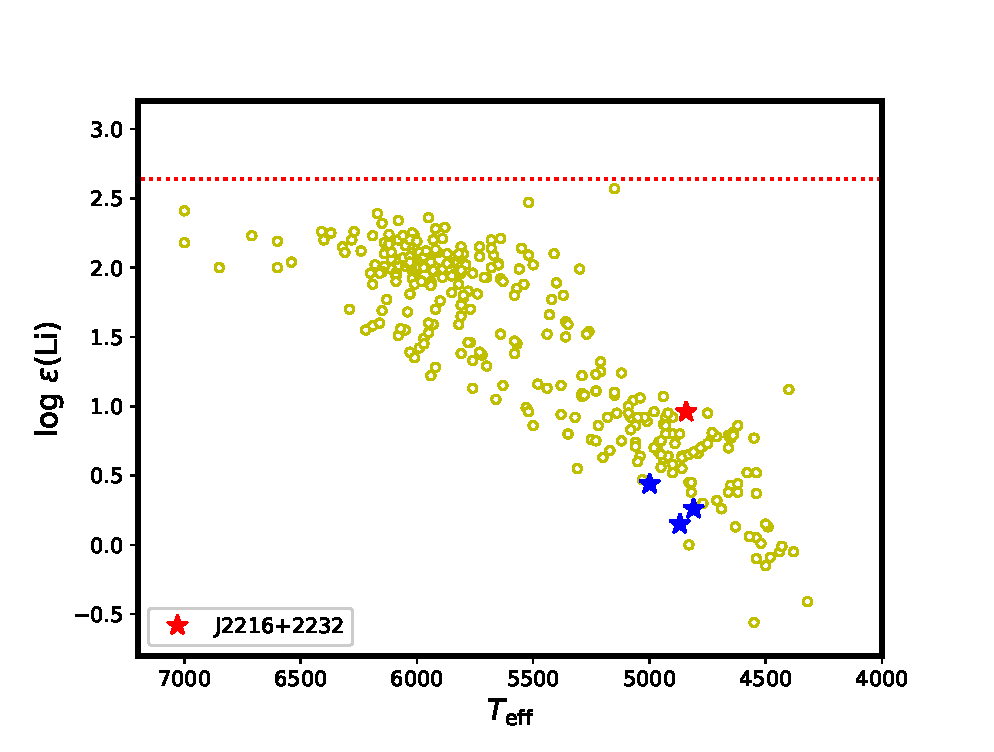
\includegraphics[width=\textwidth, angle=0]{Li_Teff_1star}
\caption{log$\epsilon$ lithium abundances as a function of effective temperature. Red filled star refers to J2216$+$2232, blue filled stars refer to the determined upper limits, and small open circles 
refer to the full sample of \citet{2014AJ....147..136R}. The dotted line 
shows the predicted primordial lithium abundance, log$\epsilon_{Li}$ = 2.64 \citep{2007ApJS..170..377S}. }
 \label{fig:Li}
\end{figure}

Lithium is considered as a key diagnostic, to test and constrain our understanding of the early Galaxy, of stellar interiors and evolution.
Figure  \ref{fig:Li} illustrates the evolution of lithium as a function of \Teff\,using the halo star sample from \citet[including upper limits]{2014AJ....147..136R}.
The dotted line refers to the primordial lithium abundance predicted by the Standard Big Bang Nucleosynthesis \citep{2007ApJS..170..377S}.
Among the program stars, we could only detect Li in 2216$+$2232 (shown as red filled star) with A(Li) = 0.95. For completeness the upper limits for 
the rest of our sample stars have been provided (blue filled stars). This is not unexpected, as our sample stars are red-giants, whose Li content in the 
outer layers have been diluted by the canonical extra mixing and the first dredge-up (FDU) process.


Our sample stars exhibit relatively high [C/Fe] ratios, as shown
in Figure \ref{fig:C_Fe_L} (left panel), which represents [C/Fe] ratio as a function of luminosity. 
We adopted a classification of \citet{2007ApJ...655..492A}, who suggest a
scheme that takes into consideration the nucleosynthesis and
mixing effects in giants. 
We define the stars that satisfy the
following criteria as CEMP stars: [C/Fe]$\geqslant$0.7 for stars with $\log$(L/L$_\odot$)$\leqslant$2.3 and 
[C/Fe]$\geqslant$3.0$-$ $\log$(L/L$_\odot$) for stars with $\log$(L/L$_\odot$)$>$2.3. The luminosities of our stars were calculated 
based on the prescription of \citet{2007ApJ...655..492A}, assuming stellar mass of 0.8 M$_\odot$, following 
\citet{2005ApJ...632..611A} and \citet{2005ApJ...635..349R}. For completeness, and due to the fact that our sample stars are gaints, we use the carbon evolutionary correction described in \citet{2014ApJ...797...21P} to assess whether our sample stars could indeed be classified as CEMP, this method suggests that carbon levels decrease as stars evolve into the giant branch phase, due to some level of internal mixing.  As a result, the correction increases the C abundances up to several dex, which support our claims that these stars are CEMP stars.




\vspace{5mm}
\begin{figure}[!ht]
\centering
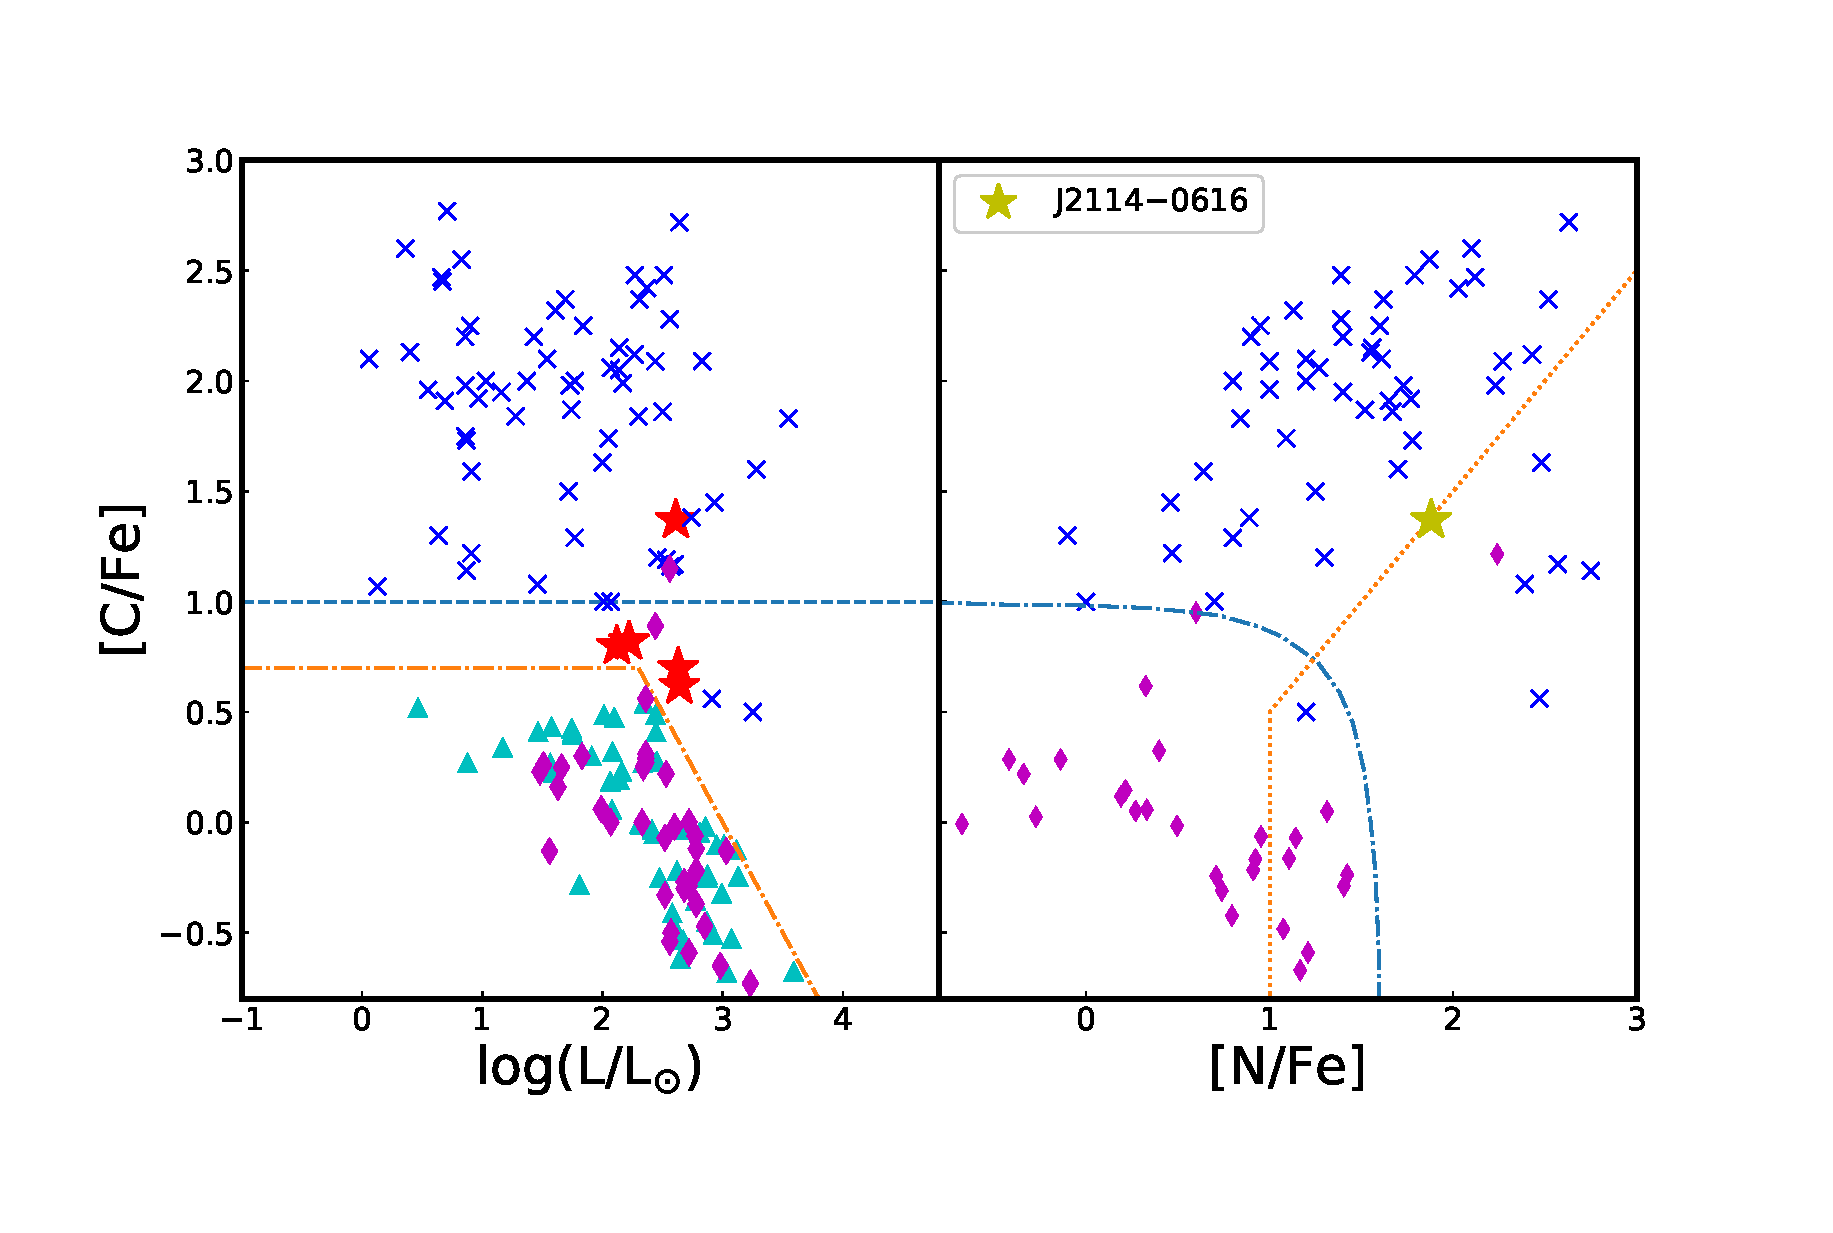
\includegraphics[width=\textwidth, angle=0]{CEMP.eps}
\caption{Left panel: [C/Fe] versus luminosity for our sample stars. The dash-dotted line indicates the dividing line between 
carbon-enhanced and carbon-normal stars as defined in \citet{2007ApJ...655..492A}. The dashed line corresponds to [C/Fe] = 1.0. 
Right panel: [C/Fe] vs. [N/Fe]. The two criteria for NEMP stars suggested by \citet{2012A&A...547A..76P} are respectively shown in dotted 
([N/Fe] $\geq$ 1.0 and [N/C] $\geq$ 0.5) and dash-dotted lines ([(C+N)/Fe] $>$ 0.9).
The filled red stars refer our sample stars. Non-carbon-enhanced objects studied by previous works \citep{2000A&A...354..169G, 2004A&A...416.1117C, 
2004ApJ...607..474H, 2005ApJ...632..611A} are shown by triangles up. Metal-poor stars from \citet{2005A&A...430..655S} (filled diamonds), 
and CEMP stars from \citet{2007ApJ...655..492A} (crosses) are also plotted for comparison. The candidate to CNEMP objects J2114-0616 is marked.}
\label{fig:C_Fe_L}
\end{figure}


With the \citet{2007ApJ...655..492A} definition of CEMP stars and the carbon evolutionary correction described in \citet{2014ApJ...797...21P} in mind, Figure \ref{fig:C_Fe_L} (left panel) shows that our program stars are located above the limit.  
Thus, we point  J1054$+$0528, J1529$+$0804, J1645$+$4357, J2114$-$0616, and J2216$+$2232 as
CEMP stars.


For most of our program stars CN bands are not measurable,
we could only measure N abundance for J2114-0616, which exhibits high nitrogen abundance with [N/Fe]=1.88, [N/C]$>$0.51, and [(C+N)/Fe]=1.53.  
Figure \ref{fig:C_Fe_L} (right panel) shows [C/Fe] as a function of [N/Fe], with the dotted and dash-doted lines referring to \citet{2012A&A...547A..76P} NEMP stars criteria.
We classify J2114$-$0616 as a potential nitrogen-enhanced metal-poor (NEMP) star.
Since J2114$-$0616 satisfies both criteria (star with [C/Fe]$\geqslant$1.0 and [N/C]$\geqslant$0.5), it can be designated as a 
carbon and nitrogen-enhanced metal-poor (CNEMP) star.  

Moreover, we investigated [Eu/Fe] as a function of [Ba/Fe] to study
s-process and r-process enrichment, under the pretext that J2114$-$0616 shows 0.0$< $ [Ba/Eu] $ <$ +0.5, and [Ba/Fe] $>$ 0.5 (see figure \ref{fig:CEMP}), we regard it as a CEMP-r/s star.
In addition to the enhancements in both slow (s-) and rapid (r-) process species, J2114$-$0616 shows high [N/Fe] ratio, along with its high [C/Fe],
 which suggest that its peculiar chemical pattern may come from mass transfer from an AGB companion, before it tuned to a white dwarf.


 
\vspace{5mm}
\begin{figure}[!ht]
\centering
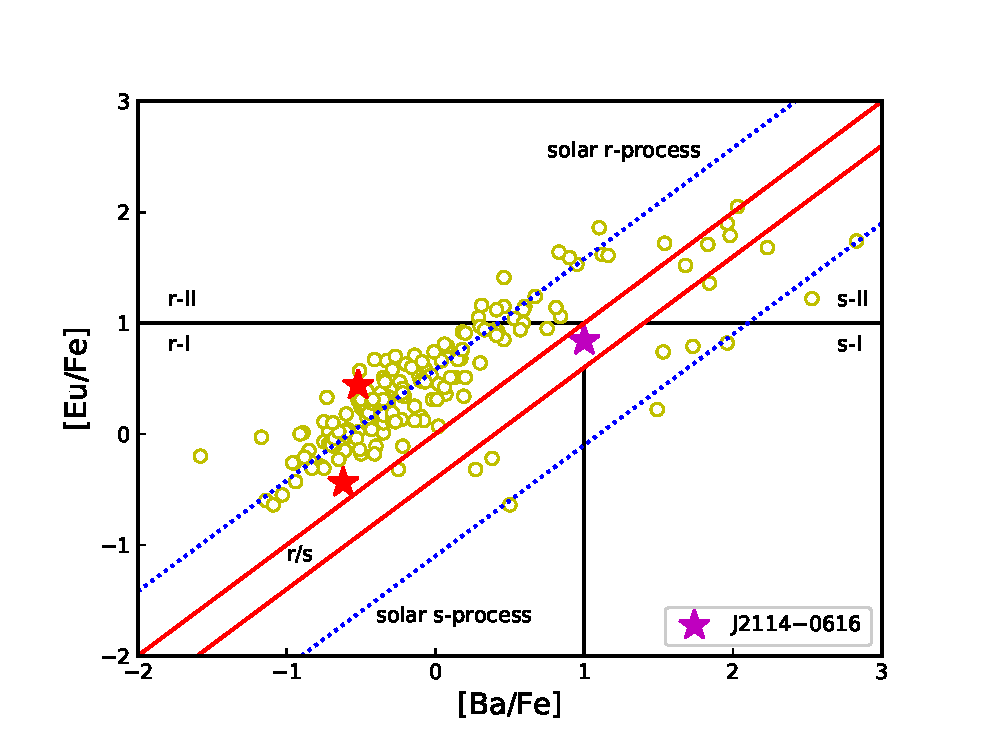
\includegraphics[width=\textwidth, angle=0]{Ba_vs_Eu.eps}
\caption{[Eu/Fe] as a function of [Ba/Fe], the open circles are data take from saga database \citep{2008PASJ...60.1159S} and the magenta star refer to the position of J2114$-$0616. }.
\label{fig:CEMP}
\end{figure}

\vspace{5mm}
\begin{figure}[!ht]
\centering
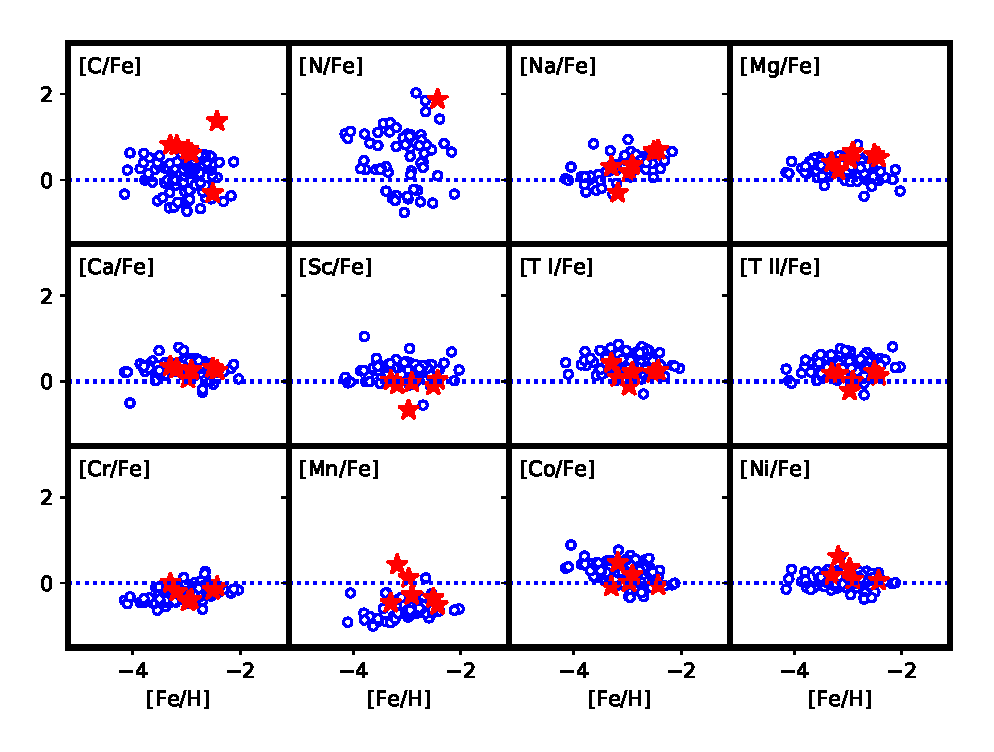
\includegraphics[width=\textwidth, angle=0]{light_elements2.eps}
\caption{Comparison between the light-element abundances in our sample stars (red filled star) and the literature C-normal metal-poor stars from \citet{2013ApJ...762...26Y}  (blue open circles).}
\label{fig:light_Fe}
\end{figure}

\vspace{5mm}
\begin{figure}[!ht]
\centering
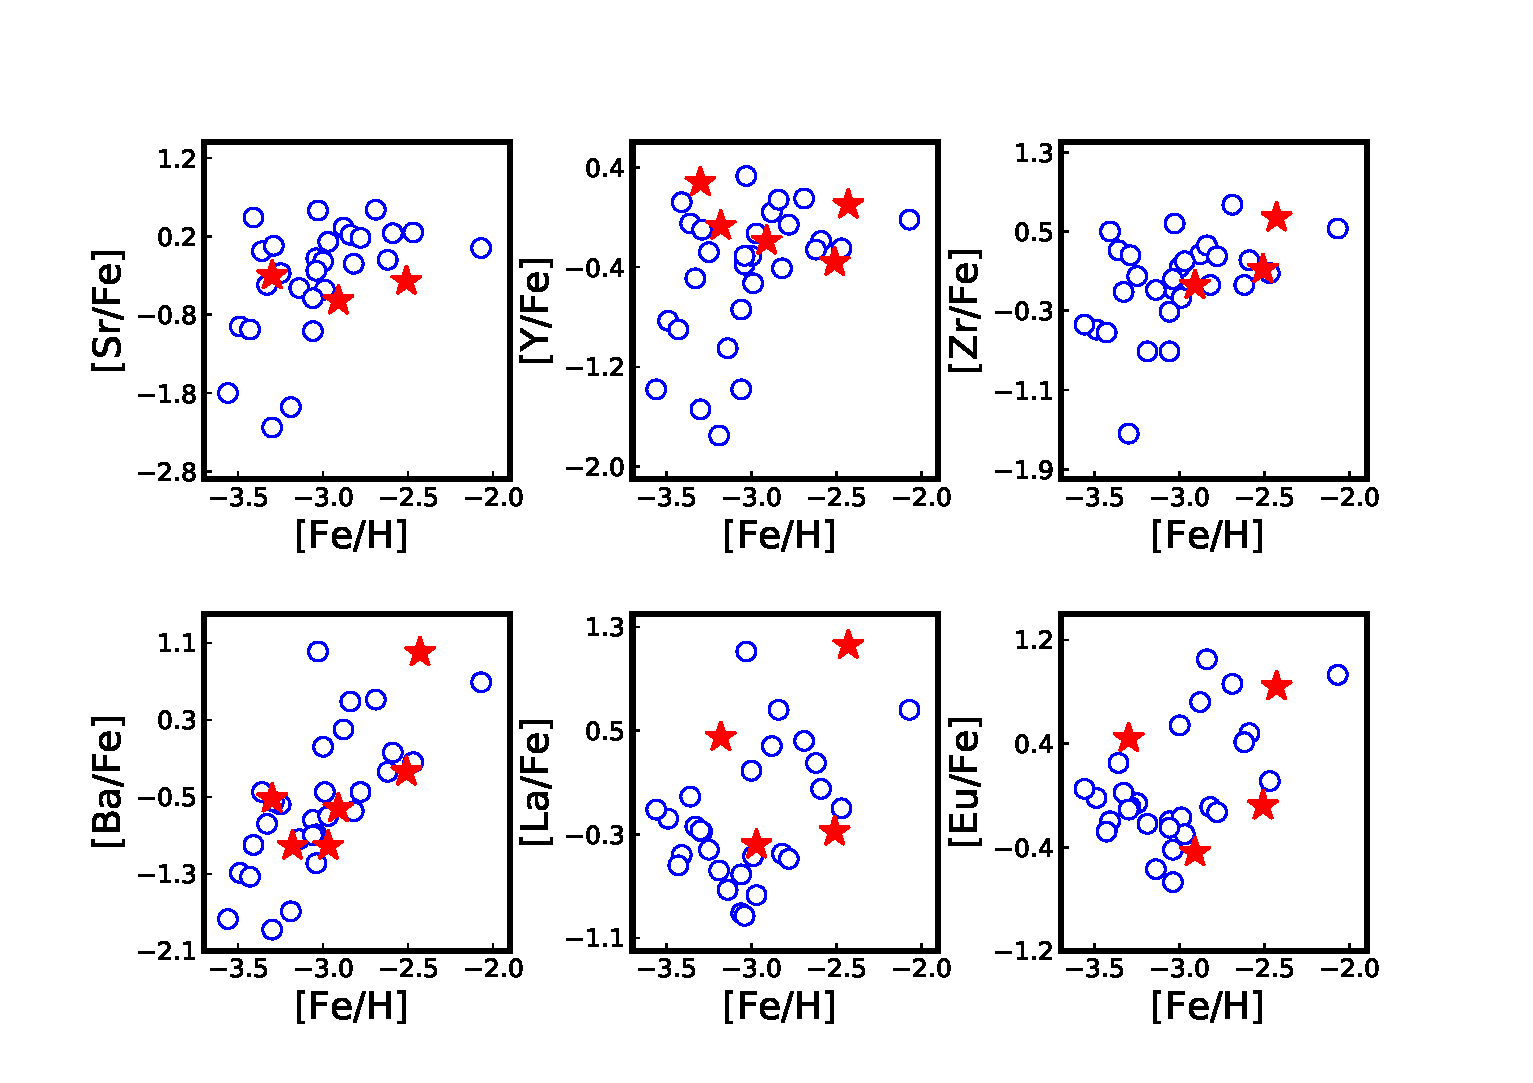
\includegraphics[width=\textwidth, angle=0]{neutron_capture.eps}
\caption{Selected neutron-capture elements abundances in our sample stars (red filled stars), as a function of metallicity, compared to literature data adopted from \citet{2007A&A...476..935F} (blue open circles).}
\label{fig:heavy_Fe}
\end{figure}

\begin{figure}[!ht]
\centering
\includegraphics[width=\textwidth, angle=0]{solar_r_s-process_all.eps}
\caption{Abundance patterns for the neutron-capture elements in our sample. The solid line represents the Solar-system s-process abundance pattern from \citet{2000ApJ...544..302B}, scaled to match the observed abundance of Ba in each star. The dotted line represents the Solar-system r-process abundance pattern from \citet{2000ApJ...544..302B}, scaled to match the observed abundance of Eu in each star. Note that we only include these stars with measured Ba and Eu.}
\label{fig:patterns}
\end{figure}



Light element distributions in CEMP stars are quite similar to those in non-carbon-enhanced stars (C-normal). The abundance ratios [X/Fe]
as a function of [Fe/H] of our sample stars (red filled stars) are presented in Figure \ref{fig:light_Fe}, for the elements from C through Zn,
compared with literature data adopted from \citet{2013ApJ...762...26Y} (blue open circles). In general, the abundance ratios seen in our sample show good agreement
with the abundance ratio trends defined by the literature sample. On the other hand, J1529+0804, which shows enhancement
in manganese with [Mn/Fe]=0.43, is not a good example of this agreement, this enhancement may also be true for J1645+4357 ([Mn/Fe]=0.12), keeping in mind that
at low metallicities, the NLTE behavior may systematically increase the manganese abundance up to 0.7 dex (which we will explore in future work) \citep[e.g.,][]{2008A&A...492..823B}.
  
\subsection{Nucleosynthetic signatures of s- and r-process}

Only elements lighter than zinc can be produced via nuclear-fusions, on the other hand, heavier
elements can be synthesized by either the rapid neutron capture process, r-process, and the slow neutron capture process, s-process
(e.g., \citealt{1994ARA&A..32..153M, 2007PhR...450...97A} and references therein). Metal-poor stars provide unique opportunities to 
attain nucleosynthetic signatures, thus better understanding of the chemical evolution of
these elements and the nucleosynthesis occurred in the early Universe.


As mentioned previously, we were able to determine abundances for up to 10 heavy elements, including the light trans-iron elements ($38\leq$Z$\leq46$) and the second r-process peak elements. 
The abundances of selected neutron-capture elements for our sample stars (red filled stars), as a function of the metallicity, overlaid with literature data adopted from \citet{2007A&A...476..935F} (blue open circles) are shown in  Figure \ref{fig:heavy_Fe}. No significant discrepancies are found between the selected neutron-capture elements abundances of our sample stars and the literature data.

Figure \ref{fig:patterns} shows the neutron-capture element abundances for HD2796 and three sample stars, compared with the Solar System s-process (normalized to Ba - solid line) and r-process (normalized to Eu - dotted line) components. The s- and r- fractions were taken from \citet{2000ApJ...544..302B}. Abundances for the first-peak s-process elements (Sr, Y, and Zr) are well described by the Solar s-process for HD2796 and J2216+2232, while for J1054+0528 and J2114-0616 they are roughly consistent with the r-process component. At the same time, the noticeable deviations from for the light elements might interestingly be related to the effects of core-collapse supernovae. In contrast, for the second-peak s-process elements, there is an excellent agreement between measurements and the Solar s-process component for J2114-0616 which, combined with its enhancements in carbon and nitrogen, supports the hypothesis of mass transfer in a binary system from an AGB companion. For J1054+0528, it appears that all the neutron-capture element abundances are a result of an r-process event, with no contributions from the s-process component.

We could only detect weak Ba II lines in the spectrum of J1645$+$4357, which results in a relatively low Ba abundance while no other s-process elements can be detected.
Such chemical patterns (high carbon, low barium, and absence of other s-process elements) suggests that J1645$+$4357 was formed out of pristine gas.
The common definition of strongly r-process-enhanced star is [Eu/Fe] $> +1.0$ and [Ba/Eu] $< 0$ and moderately r-process-enhanced star is (r-II stars) $+0.3 \geq$[Eu/Fe]$\leq +1.0$ and [Ba/Eu] $< 0$ \citep[e.g.,][]{2018ARNPS..68..237F}, 
adopting this criterion we suggest that J1054$+$0528 ([Eu/Fe]=0.44) is a new member of the moderately r-process-enhanced stars (r-I stars). On the other hand, J2114$-$0616 exhibits different chemical abundance patterns, 
enhancement of s-process species along with relatively high magnesium abundance
suggesting that $^{22}$Ne($\alpha$, n)$^{25}$Mg may have operate as a main neutron source in J2114$-$0616 \citep{2010A&A...509A..93M}.
Moreover, it turns out that the neutron density linked to this reaction favors the production of cerium (81\% synthesized by s-process) and europium (97\% synthesized by r-process),
suggesting that these elements can't be explained by s-process only, and additional r-process is required to describe this behavior \citep{1998ApJ...497..388G,2000A&A...362..599G}. 





\subsection{Kinematics and dynamics} \label{sec:kinematics}




\begin{figure}[!ht]
\begin{center}
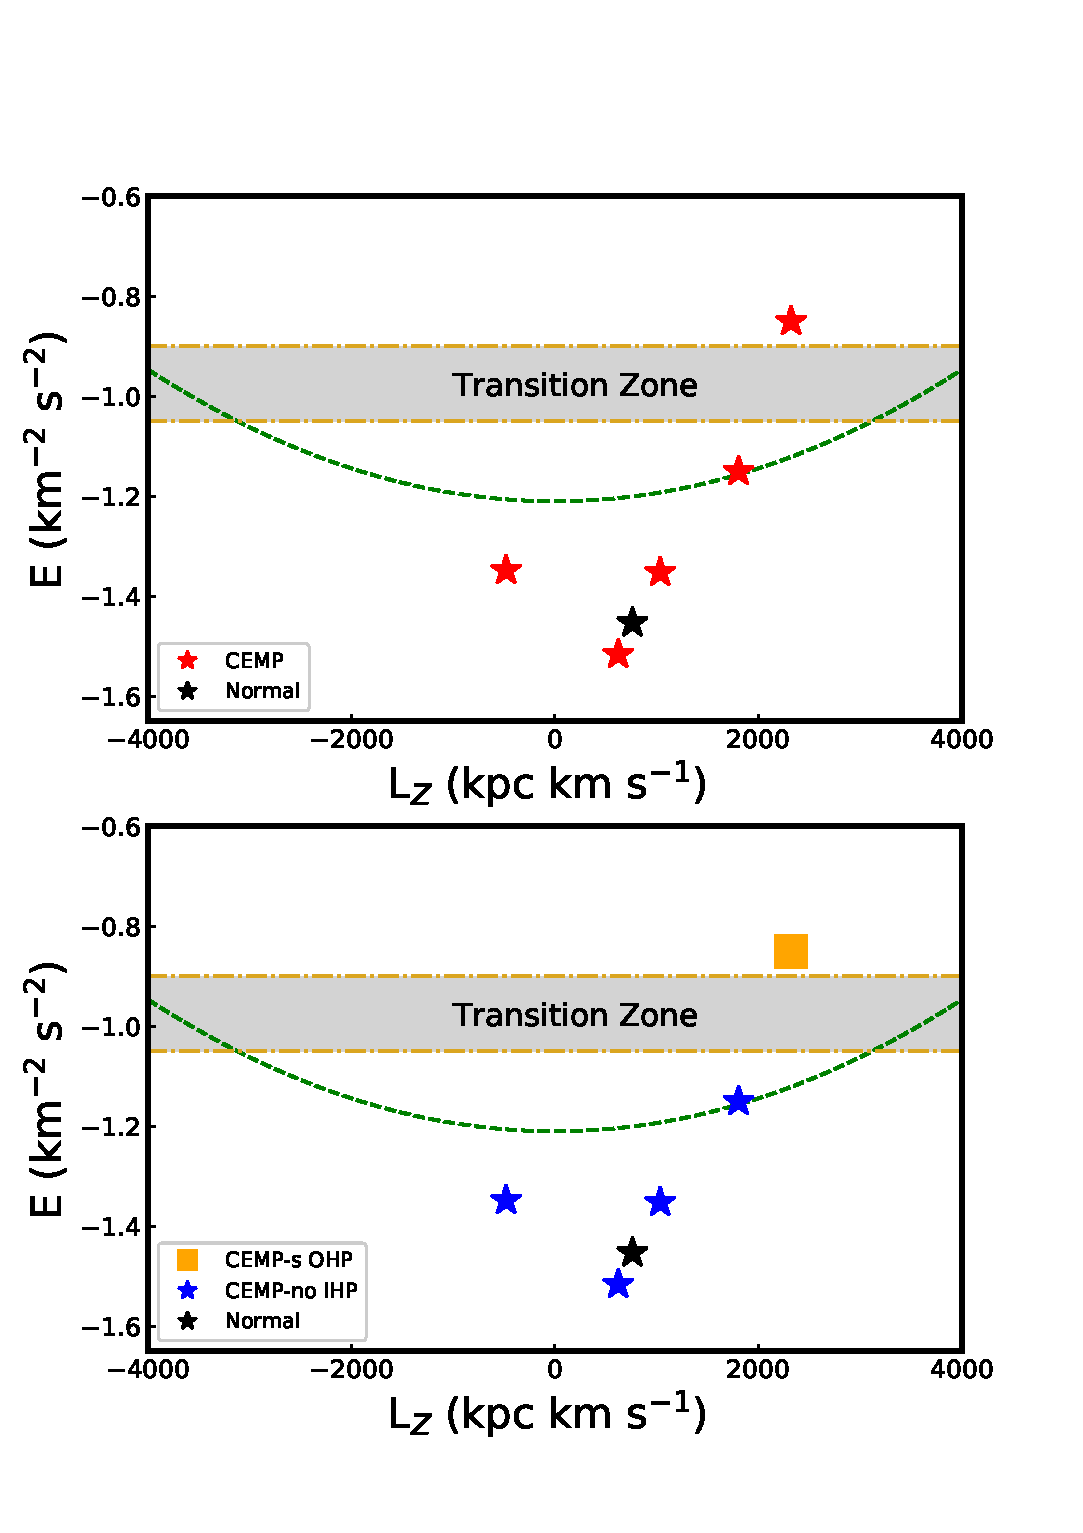
\includegraphics[scale=0.5]{vmp2.eps}\end{center}
\caption{Total energy vs. angular momentum in the z direction for the stars in our sample. Top panel: C-normal stars are represented by black
stars, while CEMP stars are denoted by red stars. Bottom panel: the same sample of stars, with blue filled star symbols indicating CEMP-no members of the inner halo, the orange filled square symbol represents the CEMP-no and CEMP-s members of
the outer halo. The green dashed curve denotes
the locus of the points that possess constant apo-Galactic radius, rapo = 15 kpc, while the golden dot-dashed horizontal lines shows the values of the energies delimiting the transition zone.}
\label{fig:apo_peri}
\end{figure}

The full space motion is derived by combining the observables obtained by Gaia DR2, positions and proper motions ($\alpha$, $\delta$, $\mu_{\alpha}$, $\mu_{\delta}$). We utilize the software {\tt TOPCAT} to cross match our sample with two catalogs from the Virtual Observatory: Gaia DR2 \citep[][for proper motions]{2018A&A...616A...1G} and Gaia DR2 distances \citep[][for distances]{2018AJ....156...58B}. Radial velocities are obtained through cross-correlation with synthetic spectra after the heliocentric corrections to the observed spectra are applied.
The velocities calculated in the Local Standard of Rest (LSR) are referred to as $(U, V, W)$ which are corrected for the motion of the Sun by adopting the values ($U, V, W$) = ($-$9,12,7) km s$^{-1}$ \citep{1981Sci...214..829M}. The velocity component $U$ is taken to be positive in the direction towards the Galactic anti-centre, the $V$ component is positive in the direction towards Galactic rotation, and the $W$ component is positive toward the north Galactic pole. We also compute the rotational velocity component about the Galactic centre in a cylindrical frame, denoted as V$_{\phi}$ , and is calculated assuming  that the LSR is on a circular orbit with a value of 220 km s$^{-1}$ \citep{1986MNRAS.221.1023K}. The orbital parameters are derived by adopting a St\"{a}ckel type gravitational potential (which consists of a flattened, oblate disk, and a nearly spherical massive dark-matter halo; a complete description is given by \citet[][Appendix A]{2000AJ....119.2843C} and integrating their orbital paths based on the starting point obtained from the observations. \\ In addition, we evaluate the integrals of motion for any given orbit, deriving the energy, E, and the angular momentum in the vertical direction, L$_{Z}$ = R x V$_{\phi}$. Note that R represents the distance from the Galactic center projected onto the disk plane. Typical errors on the orbital parameters \citep[at Zmax $<$ 50 kpc;][]{2010ApJ...712..692C} are: $\sigma$$_{rperi}$ $\sim$ 1 kpc, $\sigma$$_{rapo}$ $\sim$ 2 kpc, σ$_{ecc}$ $\sim$ 0.1, σ$_{Zmax}$ $\sim$ 1 kpc. \\
\citet{2014ApJ...788..180C} established a method for assigning the membership to the inner- and outer-halo stellar populations based on the integrals of motion (total energy and vertical angular momentum) of a large sample of SDSS/SEGUE DR7 calibration stars. Inner halo stars are mostly highly bound to the Galaxy (lower energy values, $E$ $<$ $-$1.1 km$^{2}$ s$^{-2}$) and possess orbits with apo-galactic distance r$_{\rm apo} <$ 15 kpc, while outer halo stars are less bound to the Galaxy (higher energy values, $E$ $>$ $-$0.9 km$^{2}$ s$^{-2}$ ) and possess orbits with r$_{\rm apo} >$ 15 kpc. Stars with r$_{\rm apo} >$ 15 kpc and $E$ $<$ $-$1.1 km$^{2}$ s$^{-2}$ can be also considered pure inner halo stars. In general, stars in the outer halo are dominated by retrograde orbits but can also possess rotational velocities less retrograde or higlhy prograde, due to the large velocity dispersion  of the outer halo \citep[$\sim$ 165 km s$^{-1}$;][]{2010ApJ...712..692C}. This is clearly evident in the right panel of Figure 4 in \citep{2014ApJ...788..180C} . \\
Figure \ref{fig:apo_peri} shows the total energy, E, as a function of the angular momentum in the vertical direction, L$_{Z}$, for the program stars.  In the top panel, the black filled star symbol represents HD2796, while the red filled star symbols denote the CEMP stars. The grey horizontal area shows the range of binding energy values defining the {\it transition zone} between the inner- and the outer-halo components ($-$1.1 km$^{2}$ s$^{-2}$ $ < E$ $<$ $-$0.9 km$^{2}$ s$^{-2}$), which is defined as the energy range where stars have similar probability to be members of these components. The green dashed curve represents the locus of stars possessing orbits with constant apo-galactic radius r$_{\rm apo}$ = 15 kpc. In the bottom panel the magenta star symbols denote the CEMP-no stars in the inner halo, classified according to their value of binding energy and apo-galactic distance, the CEMP-r/s star (J2114$-$0616) is represented by an orange filled square and it is member of the outer halo. \\
Figure \ref{fig:vphi} shows the galactocentric rotational velocity as a function of the metallicity for the program stars. It is interesting to note that J2114$-$0616 possesses a prograde motion (rotate in the same direction of the galactic disk) with velocities within $\sim$ 2$\sigma$ (CEMP-r/s; J2114$-$0616) of the mean rotational velocity of the outer halo population ($-$80 km s$^{-1}$). Highly prograde stars in the outer halo were also found in the sample of CEMP stars reported in \citet[; Figure 4]{2014ApJ...788..180C}.\\
Numerical cosmological simulations of MW-mass galaxies predict that stars in the inner halo of the MW formed mainly from massive subgalactic fragments that experienced an extended star formation activity \citep{2009ApJ...702.1058Z, 2011MNRAS.416.2802F, 2012MNRAS.420.2245M, 2013MNRAS.432.3391T, 2014MNRAS.439.3128T}, while outer halo stars formed predominantly in lower-mass subgalactic fragments with short or truncated star formation history 
\citep{2007Natur.450.1020C, 2010ApJ...712..692C, 2012AAS...21922206B,  2013MNRAS.432.3391T, 2014MNRAS.439.3128T, 2016NatPh..12.1170C, 2018ApJ...859L...7C}. The central regions of simulated halos (within $\sim$ 15 kpc) have an important contribution of in-situ stars (formed in the main progenitor galaxy) which have various possible origins \citep{2004ApJ...612..894B, 2009ApJ...702.1058Z,2011MNRAS.416.2802F, 2011MNRAS.415.2652H, 2013MNRAS.432.3391T, 2015MNRAS.454.3185C, 2015ApJ...799..184P, 2016MNRAS.459L..46M}. On the contrary, stars in the outer halo formed primarily in low-mass subgalactic systems which were subsequently accreted. The origin of halo stars can be understood by inspecting a combination of their orbital parameters and integrals of motion. In case of our sample, J2114$-$0616, possesses orbital parameters, energy and vertical angular momentum that place it in the outer halo population and it likely were formed in low-mass systems outside the virial radius of the progenitor galaxy and accreted later on. The orbital parameters and binding energy of the remaining CEMP stars, J1054+0528, J1529+0804, J1645+4357 and J2216+2232, suggest that they are members of the inner halo population. However, their metallicity and C-enhancement indicate that they may have formed not in situ but in small mass subgalactic fragments which were accreted very early on and contributed to the old central regions of the halo system \citep{2018MNRAS.473.1656T, 2018ApJ...859L...7C}.




\begin{figure}[!ht]
\begin{center}
\includegraphics[scale=0.5]{feha_vphi.eps}
\end{center}
\caption{Galactocentric rotational velocity vs metallicity for the program stars color coded as in Figure 12.}
\label{fig:vphi}
\end{figure}
